%%%%%%%%%%%%%%%%%%%%%%%%%
\section{\label{sec:rhs_muvt}Unbiased grand canonical ensemble ($\mu VT$) trials}
%%%%%%%%%%%%%%%%%%%%%%%%%

In this section, we will derive insertion and deletion trials in two cases.
In the first case, distinguishable particles in unscaled coordinates are considered.
In the second case, indistinguishable particles in scaled coordinates are considered.
Both cases will be shown to have identical acceptance probabilities.

%%%%%%%%%%%%%%%%%%%%%%%%%
\subsection{\label{sec:rhs_muvt_distinguishable}Grand canonical ensemble with distinguishable particles in unscaled coordinates}
%%%%%%%%%%%%%%%%%%%%%%%%%

A $\mu VT$ trial changes the number of particles of type $i$, given by $N_i$ with constant chemical potential, $\mu_i$, constant number of other particles, $N-N_i$, volume, $V$ and temperature, $T$.
The $\mu VT$ probability of a microstate is given by \cite{norman_investigation_1969, adams_grand_1975, allen_computer_1989, frenkel_understanding_2002}
\begin{equation}
\Pi(N_i) \diff\mathbf{r}^N \diff\boldsymbol{\omega}^N\propto \frac{e^{\beta\mu_i N_i - \beta U}}{\Lambda_i^{DN_i}} \diff\mathbf{r}^N\diff\boldsymbol{\omega}^N,
\label{eq:rhs_muvt_pi}
\end{equation}
where $\Lambda_i$ is the de Broglie wavelength of species $i$.
In classical computer experiments, the particles are treated as distinguishable (e.g., each particle is distinguished by an index in an ordered array).
In this case, the indistinguishable particle correction of $1/N!$ does not appear.
We will show that identical acceptance probabilities are obtained whether we treat the particles as distinguishable or indistinguishable by including the $N!$ term in an alternative derivation in the following Section~\ref{sec:rhs_muvt_alt}.

It is convenient to make Eq.~\ref{eq:rhs_muvt_pi} more compact by introducing the activity, $z_i$, of a particle of type $i$,
\begin{equation}
z_i = \frac{e^{\beta \mu_i}}{\Lambda_i^D}.
\label{eq:activity}
\end{equation}
which has the units of inverse volume and is equivalent to the ideal gas number density.
The number of particles of type $i$ in an ideal gas, $N_{i}^{\mathrm{id}}$, may be derived as the partial derivative of the grand potential with respect to the chemical potential of $i$ at constant $V$ and $T$, resulting in
\begin{equation}
N_{i}^{\mathrm{id}} = V\frac{e^{\beta \mu_i}}{\Lambda_i^D} = Vz_i.
\label{eq:gce_ideal_gas_density}
\end{equation}
Substituting Eq.~\ref{eq:activity} into Eq.~\ref{eq:rhs_muvt_pi} results in
\begin{equation}
\Pi(N_i) \diff\mathbf{r}^N \diff\boldsymbol{\omega}^N\propto z_i^{N_i} e^{-\beta U} \diff\mathbf{r}^N\diff\boldsymbol{\omega}^N.
\label{eq:rhs_muvt_pi_z}
\end{equation}
Using Eq.~\ref{eq:rhs_muvt_pi_z}, the ratio of $\mu VT$ microstate probabilities in Eq.~\ref{eq:detailed_balance} is given by
\begin{equation}
\frac{\Pi_n}{\Pi_o} = (z_i\diff\mathbf{r}\diff\boldsymbol{\omega})^{\Delta N_i} e^{-\beta\Delta U}.
\label{eq:rhs_muvt}
\end{equation}
where $\Delta N_i = N_{in} - N_{io}$, and $N_{in}$ and $N_{io}$ are the number of particles of type $i$ in the new and old microstate, respectively.
If an $NVT$ trial is attempted in the $\mu VT$ ensemble, $\Delta N_i=0$, and Eq.~\ref{eq:rhs_muvt} is reduced to Eq.~\ref{eq:rhs_nvt}.

%%%%%%%%%%%%%%%%%%%%%%%%%
\subsection{\label{sec:lhs_insdel}Insertion and deletion trials with distinguishable particles in unscaled coordinates}
%%%%%%%%%%%%%%%%%%%%%%%%%

\begin{figure}
\begin{centering}
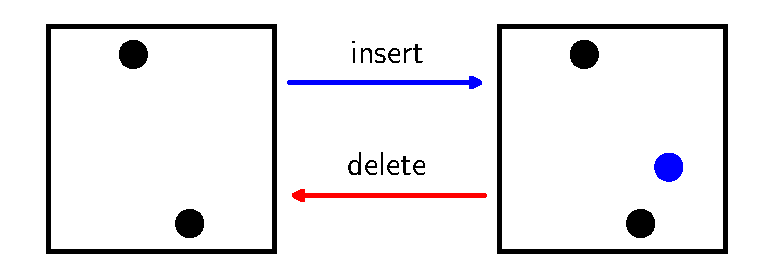
\includegraphics[width=8.5cm]{../figures/muvt.pdf}
\caption{
Insertion trials randomly add a particle, here shown in blue, uniformly within the simulation volume.
Deletion trials remove a random particle, and are the reverse of insertions.
}
\label{fig:muvt}
\end{centering}
\end{figure}

Because particle insertion and deletion trials \cite{norman_investigation_1969, adams_grand_1975} are the reverse of each other, as shown in Fig.~\ref{fig:muvt}, they must be considered together to derive the acceptance probability.
These two trials are collectively referred to as particle transfers (from an ideal gas state).
Insertion and deletion trials for particles of type $i$ proceed as follows.
First, a particle insertion or deletion trial is chosen with equal probability.\footnote{More generally, insertions may be selected with a probability of $P_{bias}$ that is not necessarily $1/2$, and deletions with a probability of $1-P_{bias}$.
In multiple places in this article, we use a $1/2$ probability for choosing between two different trials to simplify the equations.}
If a particle insertion trial is chosen, then a particle type $i$ is placed at a random position selected uniformly in the simulation volume, $V$.
If a particle deletion trial is chosen, then a particle of type $i$ is randomly chosen from among the $N_i$ particles for removal.
If multiple particle types are to be inserted and deleted, then the MC simulation could have a trial for each particle type.

In order to apply Eq.~\ref{eq:detailed_balance}, reverse trials must be considered as having occurred immediately after the forward trial.
This is important to note when deriving the probability of the reverse move, and to clarify that $N_i$ is defined at the beginning of the insertion trial.
The reverse trial deletion then has $N_i+1$ particles of type $i$, including the particle that was added during the forward transition.
Transition probabilities for insertion and deletion are not symmetric \cite{norman_investigation_1969, hastings_monte_1970}.
The transition probability of an insertion trial as the forward transition is then summarized in Table~\ref{tab:lhs_ins}.

\begin{table}
\begin{center}
\begin{tabular}{|c|c|}
 \hline
 \thead{Forward} & \thead{$\alpha_{o\rightarrow n}$} \\ [0.5ex]
 \hline
 Choose insert & $1/2$ \\
 \hline
 Choose position in $V$ & $\diff\mathbf{r}/V$ \\
 \hline
 Choose orientation & $P_{\omega n}\diff\boldsymbol{\omega}$ \\
 \hline\hline
 \thead{Reverse} & \thead{$\alpha_{n\rightarrow o}$} \\ [0.5ex]
 \hline
 Choose delete & $1/2$ \\
 \hline
 Choose particle of type $i$ & $1/(N_i+1)$ \\
 \hline
\end{tabular}
\caption{Particle insertion transition probabilities.}
\label{tab:lhs_ins}
\end{center}
\end{table}

Substituting Eq.~\ref{eq:rhs_muvt} into the first ratio in Eq.~\ref{eq:detailed_balance}, and using Table~\ref{tab:lhs_ins} for the second ratio in Eq.~\ref{eq:detailed_balance} results in
\begin{equation}
\chi = \frac{V z_i}{P_{\omega n}(N_i+1)}e^{-\beta\Delta U},
\label{eq:lhs_ins}
\end{equation}
where $P_{\omega n}=1$ (or incorporated into the definition of $z_i$) if a completely random orientation of a rigid body is chosen (see Section~\ref{sec:lhs_rotation}), or is otherwise related to the Rosenbluth factor in CB partial regrowth of the particle (as discussed in Section~\ref{sec:lhs_rotation}).

Now consider the deletion as the forward transition.
Deletion acceptance is nearly identical to what arises for the reverse of insertions, with one caveat.
With insertion as the forward transition, $N_i$ was defined at the beginning of the insertion trial (e.g., the old microstate, or before the particle was inserted).
For deletion as the forward transition, the old microstate has $N_i$ particles to choose among.
To summarize, the transition probabilities with deletion as the forward transition and insertion as the reverse is given in Table~\ref{tab:lhs_del}.

\begin{table}
\begin{center}
\begin{tabular}{|c|c|}
 \hline
 \thead{Forward} & \thead{$\alpha_{o\rightarrow n}$} \\ [0.5ex]
 \hline
 Choose delete & $1/2$ \\
 \hline
 Choose particle of type $i$ & $1/N_i$ \\
 \hline\hline
 \thead{Reverse} & \thead{$\alpha_{n\rightarrow o}$} \\ [0.5ex]
 \hline
 Choose insert & $1/2$ \\
 \hline
 Choose position in $V$ & $\diff\mathbf{r}/V$ \\
 \hline
 Choose orientation & $P_{\omega o}\diff\boldsymbol{\omega}$ \\
 \hline
\end{tabular}
\caption{Particle deletion transition probabilities.}
\label{tab:lhs_del}
\end{center}
\end{table}

Thus, the acceptance probability for deletions is given by
\begin{equation}
\chi = \frac{P_{\omega o} N_i}{Vz_i}e^{-\beta\Delta U},
\label{eq:lhs_del}
\end{equation}
where $P_{\omega o}=1$ (or incorporated into the definition of $z_i$) if rigid bodies are inserted with random orientations (using quaternions, as discussed in Section~\ref{sec:lhs_rotation} and \ref{sec:unit_sphere}), or otherwise related to the Rosenbluth factor in CB \cite{frenkel_understanding_2002}.
Code Block~\ref{sim:ideal_gas_muvt} uses Eqs.~\ref{eq:lhs_ins} and \ref{eq:lhs_del} for an ideal gas to compare against theory, Eq.~\ref{eq:gce_ideal_gas_density}.

\begin{figure}
\lstinputlisting[
language=Python,
label={sim:ideal_gas_muvt},
caption={MC $\mu VT$ simulation of an ideal gas using Python 3, and the statistics module is provided in Section~\ref{sec:block_av}.}
]{../codes/ideal_gas_muvt.py}
\end{figure}

%%%%%%%%%%%%%%%%%%%%%%%%%
\subsection{\label{sec:rhs_muvt_alt}Grand canonical ensemble with indistinguishable particles in scaled coordinates}
%%%%%%%%%%%%%%%%%%%%%%%%%

Consider an alternative approach that includes the indistinguishable particle $N!$ correction, and uses scaled coordinates, as described in Ref.~\cite{frenkel_understanding_2002}.
In this case, the $\mu VT$ microstate probability is
\begin{equation}
\Pi(N_i)\diff\mathbf{s}^{N}\diff\boldsymbol{\omega}^{N} \propto \frac{V^{N}z_i^{N_i}}{N!} e^{-\beta U} \diff\mathbf{s}^{N}\diff\boldsymbol{\omega}^{N}.
\end{equation}
The ratio of $\mu VT$ microstate probabilities for the special case of indistinguishable particles and scaled coordinates is then
\begin{equation}
\frac{\Pi_n}{\Pi_o} = \frac{N_{io}!}{N_{in}!}\left(V z_i\diff\mathbf{s}\diff\boldsymbol{\omega}\right)^{\Delta N_i}e^{-\beta\Delta U},
\label{eq:rhs_muvt_alt}
\end{equation}
and is valid for changing the number of indistinguishable particles and choosing a newly inserted particle position in scaled coordinates, $\mathbf{s}$, not $\mathbf{r}$.


%%%%%%%%%%%%%%%%%%%%%%%%%
\subsection{\label{sec:lhs_insdel_alt}Insertion and deletion trials with indistinguishable particles in scaled coordinates}
%%%%%%%%%%%%%%%%%%%%%%%%%

As opposed to deriving insertion and deletion acceptances with distinguishable particles in non-scaled coordinates, as in Sections~\ref{sec:rhs_muvt_distinguishable} and \ref{sec:lhs_insdel}, consider a similar trial conducted with indistinguishable particles in scaled coordinates, as in Ref.~\cite{frenkel_understanding_2002}.
In this case, the first ratio in Eq.~\ref{eq:detailed_balance} is given by Eq.~\ref{eq:rhs_muvt_alt}.
But since the transition probabilities also change, the same acceptances are nonetheless obtained.

The insertion and deletion trial proceeds as follows.
First, a particle insertion or deletion trial is randomly chosen with equal probability.
If a particle insertion is chosen, then a particle of a given type $i$ is placed at a random position selected uniformly in the scaled coordinates with a probability of $\diff\mathbf{s}$.
If a particle deletion is chosen, then a random particle of a given type is chosen for removal.
Because the particles are indistinguishable, the probability associated with the selection of a particle is $1$.
The forward and reverse transitions are summarized in Table~\ref{tab:lhs_insdel_alt}.

\begin{table}
\begin{center}
\begin{tabular}{|c|c|}
 \hline
 \thead{Forward} & \thead{$\alpha_{o\rightarrow n}$} \\ [0.5ex]
 \hline
 Choose insert & $1/2$ \\
 \hline
 Choose position in scaled coordinates & $\diff\mathbf{s}$ \\
 \hline
 Choose orientation & $P_{\omega n}\diff\boldsymbol{\omega}$ \\
 \hline\hline
 \thead{Reverse} & \thead{$\alpha_{n\rightarrow o}$} \\ [0.5ex]
 \hline
 Choose delete & $1/2$ \\
 \hline
 Choose from indistinguishable particles & $1$ \\
 \hline
\end{tabular}
\caption{Alternative particle insertion transition probabilities.}
\label{tab:lhs_insdel_alt}
\end{center}
\end{table}

The product of the first and second ratios in Eq.~\ref{eq:detailed_balance} is then identical to Eq.~\ref{eq:lhs_ins} because the first ratio from Eq.~\ref{eq:rhs_muvt_alt} now supplies the terms missing from the second ratio.
Thus, the use of indistinguishable particles and scaled coordinates shifts the terms from the transition probabilities to the microstate probabilities.
Although either approach is equally valid, the remainder of this article uses distinguishable particles, as implemented in computer simulations, and $\mu VT$ derivations will use unscaled coordinates as described in Section~\ref{sec:rhs_muvt_distinguishable}, and not Section~\ref{sec:rhs_muvt_alt}.
